\documentclass[10pt]{standalone}
\usepackage{amsmath}
\usepackage{pgf,tikz}
\usepackage{mathrsfs}
\usetikzlibrary{arrows}
\pagestyle{empty}

\begin{document}

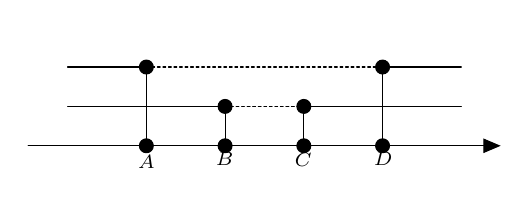
\begin{tikzpicture}[line cap=round,line join=round,>=triangle 45,x=1.0cm,y=1.0cm]

\draw[->] (0.5,0.) -- (6.5,0.);

\clip(0.5,-0.5) rectangle (6.5,1.5);
\draw  (2.,1.)-- (2.,0.);
\draw  (5.,1.)-- (5.,0.);
\draw  (4.,0.5)-- (4.,0.);
\draw  (3.,0.5)-- (3.,0.);
\draw  (1.,0.5)-- (3.,0.5);
\draw [dash pattern=on 1pt off 1pt] (3.,0.5)-- (4.,0.5);
\draw  (4.,0.5)-- (6.,0.5);
\draw  (1.,1.)-- (2.,1.);
\draw [dash pattern=on 1pt off 1pt] (2.,1.)-- (5.,1.);
\draw  (5.,1.)-- (6.,1.);
\begin{scriptsize}
\draw [fill=black] (2.,0.) circle (2.5pt);
\draw[color=black] (1.9997945151631586,-0.20608837653635753) node {$A$};
\draw [fill=black] (3.,0.) circle (2.5pt);
\draw[color=black] (2.9967784077853206,-0.17170962161835202) node {$B$};
\draw [fill=black] (4.,0.) circle (2.5pt);
\draw[color=black] (3.9937623004074823,-0.18030431034785338) node {$C$};
\draw [fill=black] (5.,0.) circle (2.5pt);
\draw[color=black] (5.007935570488647,-0.16311493288885062) node {$D$};
\draw [fill=black] (3.,0.5) circle (2.5pt);
\draw [fill=black] (4.,0.5) circle (2.5pt);
\draw [fill=black] (2.,1.) circle (2.5pt);
\draw [fill=black] (5.,1.) circle (2.5pt);
\end{scriptsize}
\end{tikzpicture}
\end{document}